\documentclass[12pt]{report}
\usepackage[utf8]{inputenc}
\usepackage{multicol}
\usepackage{xcolor}
\usepackage{tikz}
\usepackage{subfigure}
\usepackage{caption}
\usepackage{lipsum}
\usepackage[utf8]{inputenc}
\usepackage{graphicx}
\usepackage{titlesec}
\usepackage[bookmarks,breaklinks,colorlinks=true,allcolors=blue]{hyperref}
\usepackage{listings}
\usepackage{inconsolata}
\usepackage{float}
\usepackage{eso-pic}
\usepackage{comment}
\usepackage[framemethod=tikz]{mdframed}

%\usepackage{natbib}
%\bibliographystyle{plainnat}
%\setcitestyle{numbers,open={[},close={]}} 
%\AtBeginDocument{
%  \renewcommand{\bibsection}{\chapter{\bibname}}
%} % Bibliography in numbered chapter
%%

\usepackage[
backend=biber,
style=numeric,
sorting=none
]{biblatex}
\addbibresource{bibliography.bib}

\usepackage{geometry}
\usepackage{amsmath}
\usepackage{bbm}
\usepackage{parskip}
\usepackage[official]{eurosym}
\setlength {\marginparwidth }{2cm} 
\usepackage{todonotes}
\usepackage{csquotes}

\usepackage{rotating}
\usepackage{lmodern}
\usepackage{setspace}

\usepackage{enumitem}
\usepackage{wrapfig}

\usepackage[english]{babel}
\usepackage{fancyhdr}
\usepackage{hyperref}
\usepackage{soul}

\usepackage{ifthen}
\newboolean{firstanswerofthechapter}  
\usepackage{chngcntr}
\usepackage{stackengine}

\usepackage{tasks}
\newlength{\longestlabel}
\settowidth{\longestlabel}{\bfseries viii.}
\settasks{label=\roman*., label-format={\bfseries}, label-width=\longestlabel,
item-indent=0pt, label-offset=2pt, column-sep={10pt}}



\titleformat{\section}[block]{\normalfont\huge\bfseries}{\thesection.}{.5em}{\Huge}[{}]

% code formatting with listing
\lstset{
  basicstyle=\ttfamily,
  breaklines=true,
}
% Margins
\geometry{
    a4paper,
    margin=2.75cm
}
% Index depth limit
\setcounter{tocdepth}{2}
% Paragraph Indentation
\setlength{\parindent}{1cm}

\renewcommand{\lstlistingname}{Code extraction}
\renewcommand*{\lstlistlistingname}{Code Excerpts Index}

% style for chapter and section names
% see also https://texblog.org/2012/07/03/fancy-latex-chapter-styles/
\usepackage[T1]{fontenc}
\usepackage{titlesec, blindtext, color}
\definecolor{gray75}{gray}{0.75}
\definecolor{gray45}{gray}{0.45}
\definecolor{gray25}{gray}{0.25}
\definecolor{unipd}{HTML}{870011}
\newcommand{\hsp}{\hspace{20pt}}
\titleformat{\chapter}[hang]{\Huge\bfseries}{\textcolor{gray45}{\thechapter}\hsp\textcolor{gray75}{|}\hsp}{0pt}{\Huge\bfseries\textcolor{unipd}}[\color{unipd}{\titlerule[1.8pt]}]

\newcommand{\resp}[1]{\vspace{-1.5truecm}\noindent\textcolor{unipd}{\textbf{Task leader(s):}}~\emph{#1}}
\newcommand{\authors}[1]{\begin{scriptsize}\textcolor{unipd}{\textbf{Credits:}} #1\end{scriptsize}}
\newcommand{\startsolution}{\vspace{0.35truecm}\noindent\textcolor{unipd}{\textbf{Risoluzione del problema}}\vspace{0.35truecm}}
\newcommand{\solutionpoint}[1]{\noindent\textbf{Q#1.}~}

\pagestyle{fancy}
\renewcommand{\footrulewidth}{0.2pt}% default is 0pt
\renewcommand{\headrulewidth}{0.2pt}% default is 0pt
\fancyhf{}
\rhead{\bfseries \textcolor{unipd}{\emph{PoCN}}}
\lhead{\bfseries \textcolor{unipd}{\thepage}}
\lfoot{\bfseries \footnotesize\textcolor{unipd}{Project Report}}
\rfoot{\bfseries \footnotesize\textcolor{unipd}{\today}}

\newcommand\setItemnumber[1]{\setcounter{enumi}{\numexpr#1-1\relax}}

% boxes
\usepackage{fancybox}
\usepackage[framemethod=tikz]{mdframed}
\usetikzlibrary{calc}
\usepackage{chngcntr}


\makeatother


\begin{document}
    \begin{center}

\vspace*{1cm}

\begin{figure}
  \raggedleft
  \begin{minipage}{4cm}
  
\includegraphics[width=6cm]{images/logo.png}
  \end{minipage}
\end{figure}

\begin{figure}[H]
    \centering
    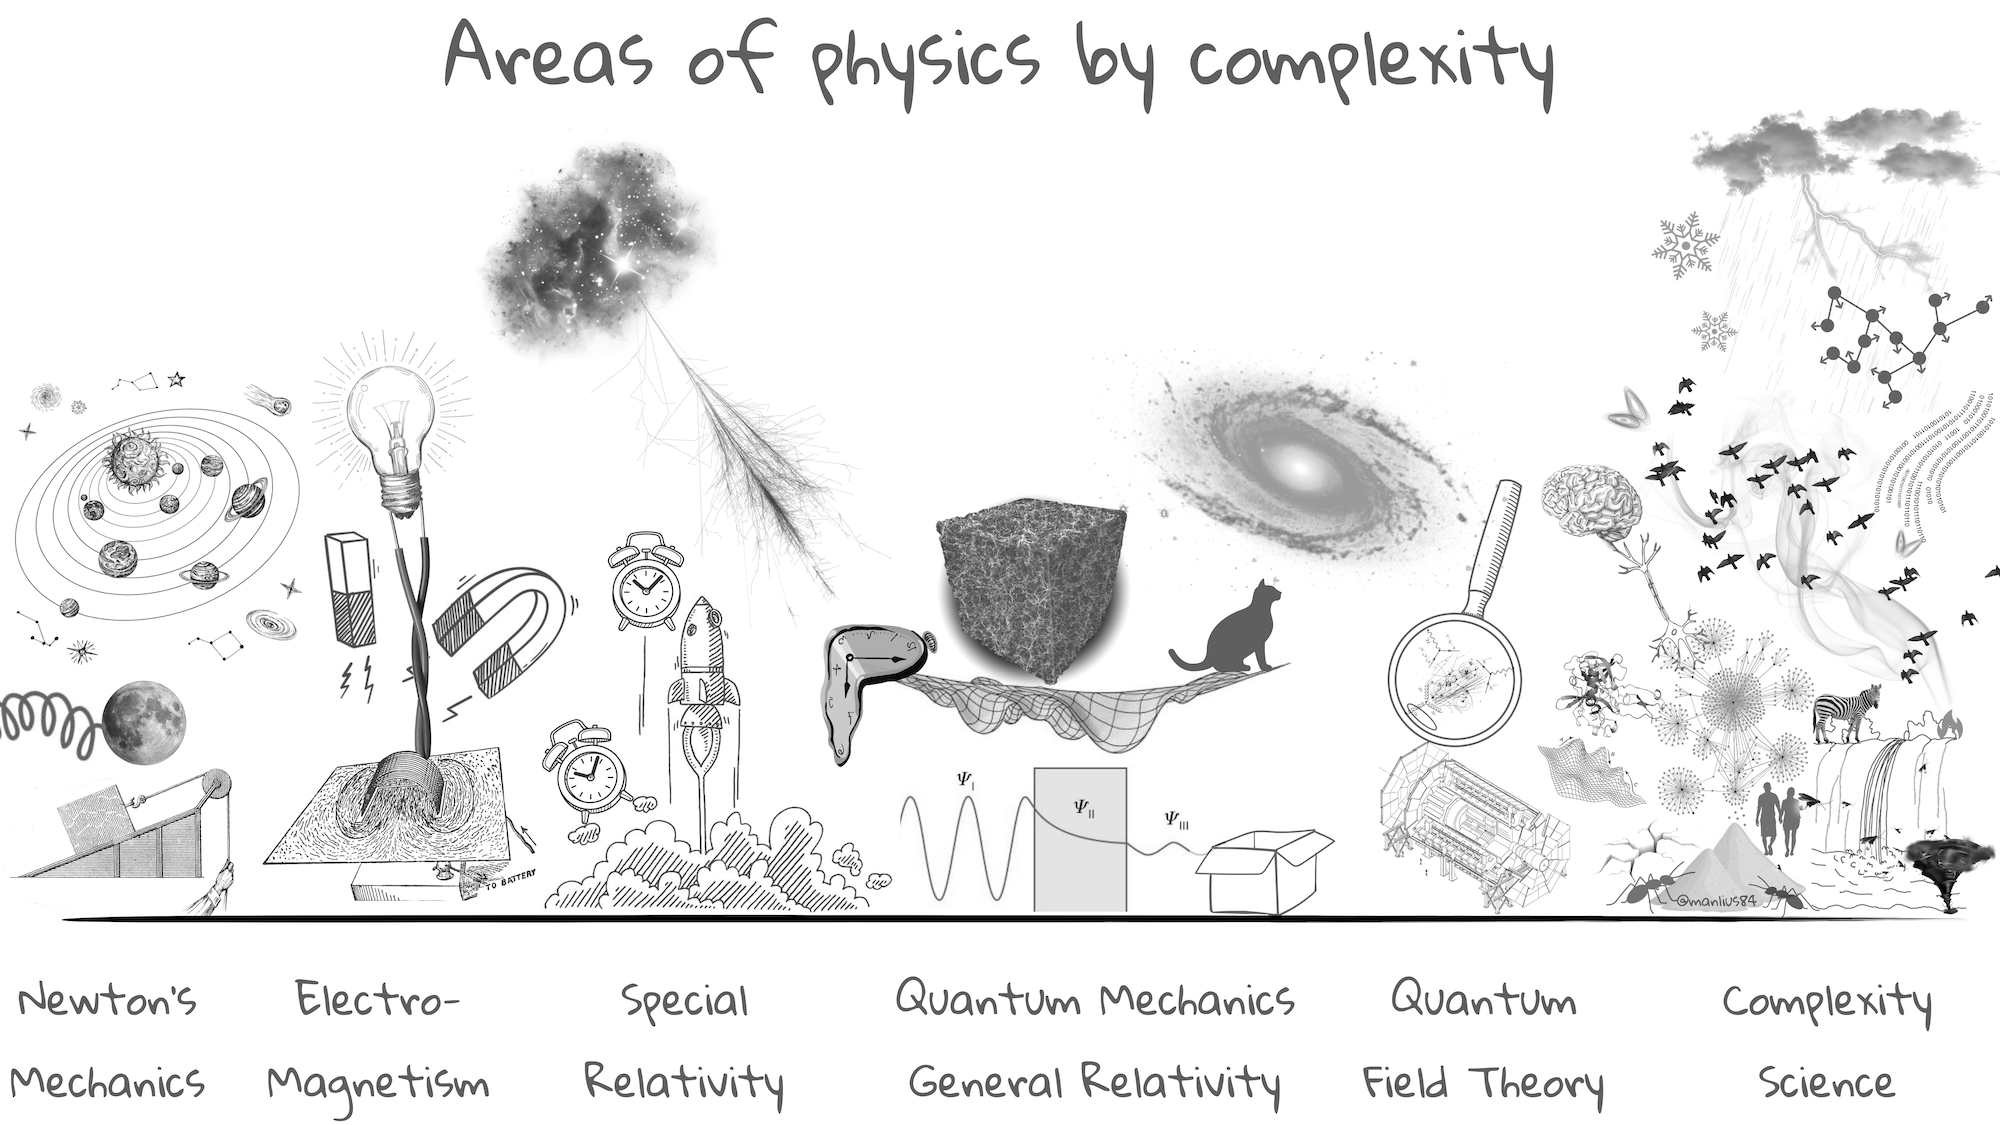
\includegraphics[width=\textwidth]{images/areas_of_physics.png} 
\end{figure}
\vspace*{1cm}
\textcolor{unipd}{\textbf{\large Physics of Complex Networks: Structure and Dynamics}} \\
\vspace*{1cm}
\textcolor{unipd}{\textbf{\huge Final Report}} \\
\vspace*{2cm}
\textbf{Student:} Zara Miriam \hfill \textbf{Last update}: \today\\
\end{center}



\thispagestyle{empty} % Prevents page number from being included on the cover
\clearpage\setcounter{page}{1} % Start including page numbers from here
\pagenumbering{roman} % in roman numerals
    
    % Index of the document and figures
    \begingroup
        % Links are normally blue, but indexes are set to black
        % so that everything does not appear blue
        \hypersetup{linkcolor=black}
        \tableofcontents
        %\listoffigures % uncomment to display list of code 
        %\lstlistoflistings % uncomment to display list of code 
        %\listof{example}{Lista degli esempi}
        %check https://tex.stackexchange.com/questions/16494/generating-lists-of-custom-environment
    \endgroup
       %Change page number style to normal
       \clearpage\pagenumbering{arabic}
    
% Sections and chapters
\titleformat{\section}[hang]{\large\bfseries}{\textcolor{unipd}{\thesection}\hsp\textcolor{gray75}{|}\hsp}{0pt}{\large\bfseries\textcolor{gray25}}[\color{unipd}{\titlerule[1.0pt]}]
% Subsection
\titleformat{\subsection}[hang]{\large\bfseries}{\textcolor{unipd}{\thesubsection}\hsp\textcolor{gray75}{|}\hsp}{0pt}{\large\bfseries\textcolor{gray25}}[\color{unipd}{}]




\chapter{Turing Patterns on Networks}
    \section{Task Description}
The goal of this task is to analyze a reaction-diffusion (Turing) dynamics on networks, with specific suggestion to replicate the results found in \cite{main_network}. 

A system governed by a reaction-diffusion mechanism can exibit pattern emergence when perturbed from an initial linearly stable equilibrium state. The conditions for pattern initiation are found through linear stability analysis. The subsequent evolution of the pattern is non-linear and eventually results in a steady state (that can be either stationary or time dependent).

The authors of \cite{main_network} described mathematically and with simulations both the pattern initiation and its subsequent non-linear evolution to the steady state. In order to keep the workload manageable for this project, I made the choice to focus only on \textbf{pattern initiation}, but do it in full mathematical detail.

    \chapter{Task title...}

\resp{Author name(s)...}

\emph{
Structure as\footnote{Remove this part from the report}:
\begin{itemize}
\item A short (max 1 page) explanation of the task, including references. Include mathematical concepts.
\item Max 2 pages for the whole task (including figures)
\item It is possible to use appendices for supplementary material, at the end of the report. Max 5 pages per task
\end{itemize}
A total of 3 pages + 5 supplementary pages per task
}

\section{A section...}
 
Reference examples: book~\cite{barrat2008dynamical}, article~\cite{de2013mathematical}, website~\cite{weforumProtectingCritical}

\section{Another section...}



\newpage
    \chapter{Task title...}

\resp{Author name(s)...}

\emph{
Structure as\footnote{Remove this part from the report}:
\begin{itemize}
\item A short (max 1 page) explanation of the task, including references. Include mathematical concepts.
\item Max 2 pages for the whole task (including figures)
\item It is possible to use appendices for supplementary material, at the end of the report. Max 5 pages per task
\end{itemize}
A total of 3 pages + 5 supplementary pages per task
}

\section{A section...}
 
Reference examples: book~\cite{barrat2008dynamical}, article~\cite{de2013mathematical}, website~\cite{weforumProtectingCritical}

\section{Another section...}



\newpage
    \chapter{Appendix}
\section{Turing Patterns in a continuous medium}

This section contains an elementary introduction to reaction-diffusion systems for pattern formation. 

An activator- inhibitor system is described by the following set of equations:

\begin{equation}
\begin{cases}
\frac{\partial}{\partial t} u(\mathbf{x}, t) = f(u, v) + D_{\text{act}} \nabla^2 u(\mathbf{x}, t) \\
\frac{\partial}{\partial t} v(\mathbf{x}, t) = g(u, v) + D_{\text{inh}} \nabla^2 v(\mathbf{x}, t)
\end{cases}
\end{equation}

where $u(\mathbf{x},\, t)$ is the local density of the activator and $v(\mathbf{x},\, t)$ is the local density of the inhibitor. $D_u$  and $D_v$ are the diffusion coefficients of the ligands or morphogens. The reactions are encoded in the functions $f(u,\,v)$ and $g(u,\,v)$. There are several choices for $f(u,\,v)$ and $g(u,\,v)$ that are able to generate patterns. Among the most studied are the Schnakenberg (1979) and the Gieger-Meinhardt (1972) kinetics (see \citep{murray}).
Whatever kinetics we might choose, it needs to meet the following basic requirements:
\begin{enumerate}
	\item Existence of a homogeneous, linearly stable equilibrium $(\overline{u},\, \overline{v})$ in absence of diffusion:
		$$
		\centering
		\begin{pmatrix}
			u(\mathbf{x},\, t) \\
			v(\mathbf{x},\, t)
		\end{pmatrix} = 
		\begin{pmatrix}
			\overline{u} \\
			\overline{v}
		\end{pmatrix}
		\quad \text{where} \quad f(\overline{u}\,, \overline{v}) = g(\overline{u}\,, \overline{v})=0 \quad \text{and, given that}
		$$
		$$
		 \quad J_{F}(\overline{u}\,, \overline{v}) := 
		\begin{pmatrix}
 			f_u & f_v \\
 			g_u & g_v
 		\end{pmatrix}, \quad
 		\begin{cases}
 			\text{tr}(J_F)= f_u + g_v < 0\\
 			\text{det}(J_F) = f_u\cdot g_v f_v\cdot g_u>0
 		\end{cases}
		\text{(linear stability)}
		$$
	\item Correct behaviour in the neighborhood of the fixed point $(\overline{u},\, \overline{v})$:
	\item Diffusion-Driven Instability
\end{enumerate}
 Qualitatively, those functions should describe the following facts:
\begin{itemize}
    \item the activator $u$ enhances its own production and the production of the inhibitor $v$;
    \item the inhibitor $v$ suppresses the production of both the activator $u$ and itself,
\end{itemize}

\begin{figure*}
	\centering
	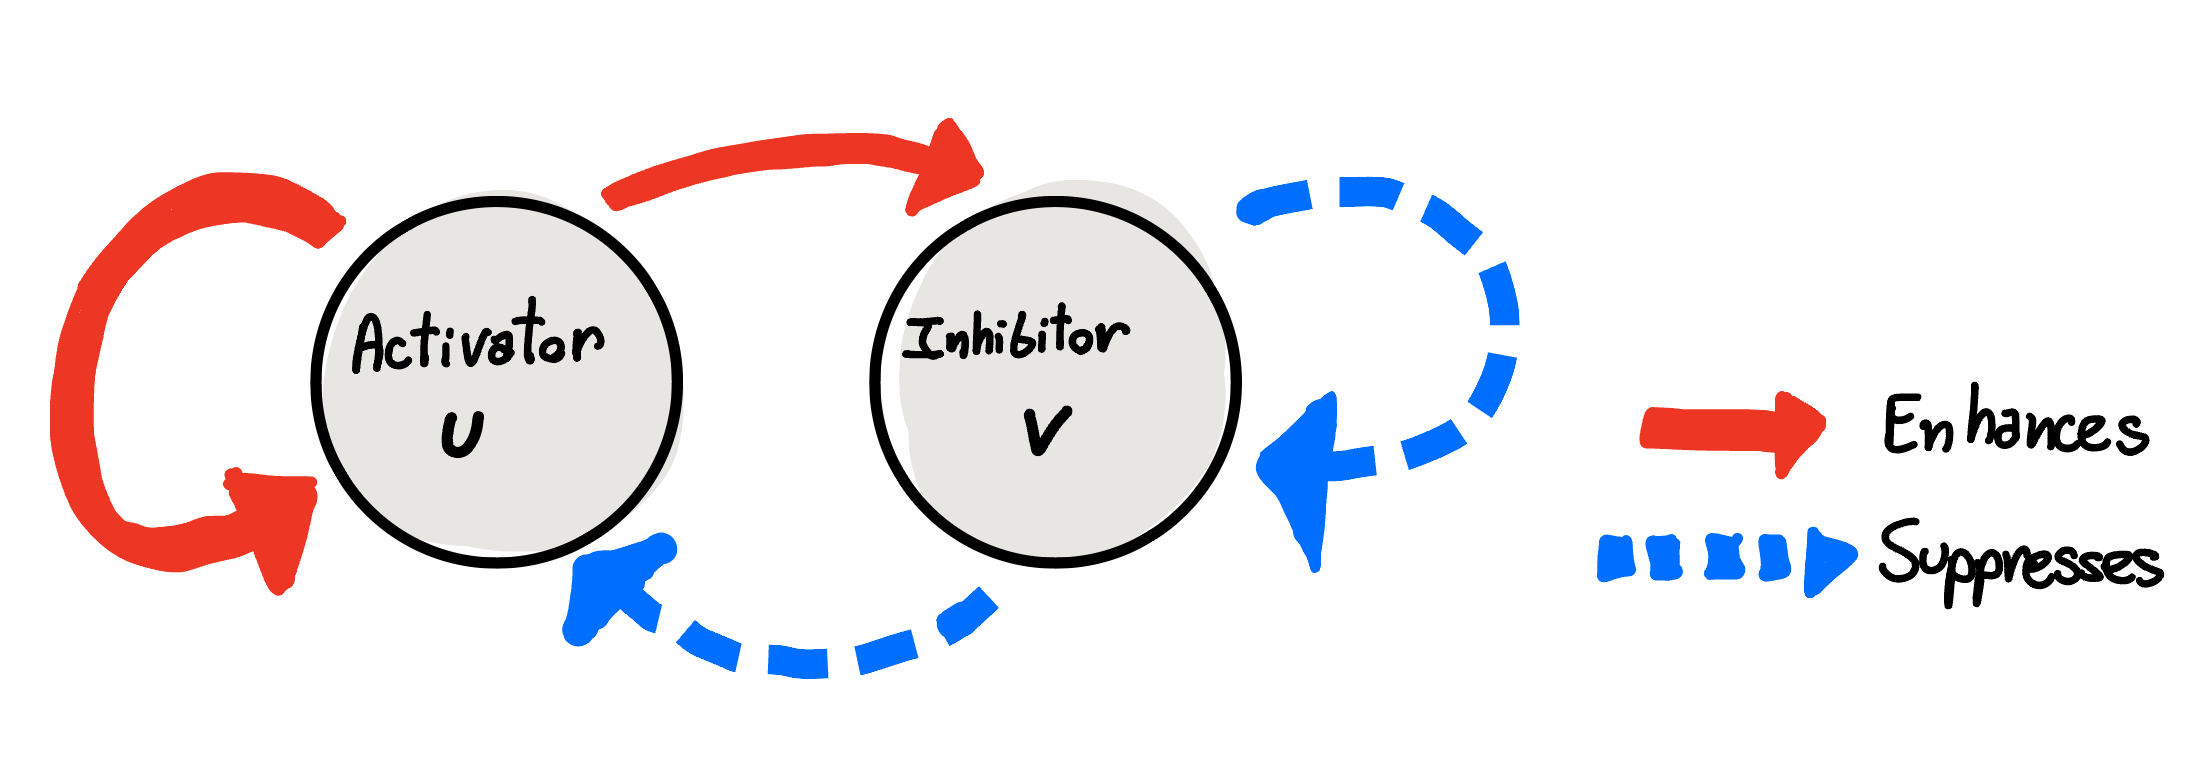
\includegraphics[width = 0.6\textwidth]{images/diagram.jpeg}
	\caption{A state diagram of the reactions}
\end{figure*}

Mathematically, these conditions translate to the following relations on the partial derivatives:
\begin{equation*}
    \begin{cases}
        \frac{\partial f}{\partial u} > 0 \,,\quad \frac{\partial f}{\partial v} < 0 \\
         \frac{\partial g}{\partial u} > 0 \,,\quad \frac{\partial g}{\partial v} < 0 \\       
    \end{cases}
\end{equation*}
It is required that, in absence of diffusion, a uniform stationary state exists, i.e.
$(\overline{u}\,, \overline{v})$
where $f(\overline{u}\,, \overline{v}) = g(\overline{u}\,, \overline{v})=0$. 

$$
\rightarrow
\begin{pmatrix}
  u(\mathbf{x}, t) \\
  v(\mathbf{x}, t) 
\end{pmatrix}
= 
\begin{pmatrix}
  \overline{u} \\
  \overline{v}
\end{pmatrix}
\quad \forall \, \mathbf{x},\, t
$$

Also, it is required that this equilibrium is linearly stable under the effect of small perturbations. Indeed, the key idea of the Turing model is that the instability is driven by diffusion, and appears only above a certain threshold function of the diffusion parameters. 


 The linear stability requirement is satisfied if the jacobian matrix of $F(u,v) = (f(u,v), g(u,v))$ evaluated at the fixed point $(\overline{u}\,, \overline{v})$, $J_F(\overline{u},\, \overline{v})$, has all eigenvalues with negative real parts $\mathcal{R}e(\lambda_i)<0$. Say 
 \begin{equation*}
 		J_{F}(\overline{u}\,, \overline{v}) := \begin{pmatrix}
 			f_u & f_v \\
 			g_u & g_v
 		\end{pmatrix}
 \end{equation*}
Then
$$
Re\{\lambda_i\} <0 \iff 	J_{F}(\overline{u}\,, \overline{v})< 0\quad  \text{(neg. def.)} \iff \begin{cases}
		\text{tr}(J_F) < 0 \\
		\text{det}(J_F)>0
	\end{cases}
	\iff \begin{cases}
		f_u + g_v < 0 \\
		f_u\cdot g_v - f_v\cdot g_u>0
	\end{cases}
$$



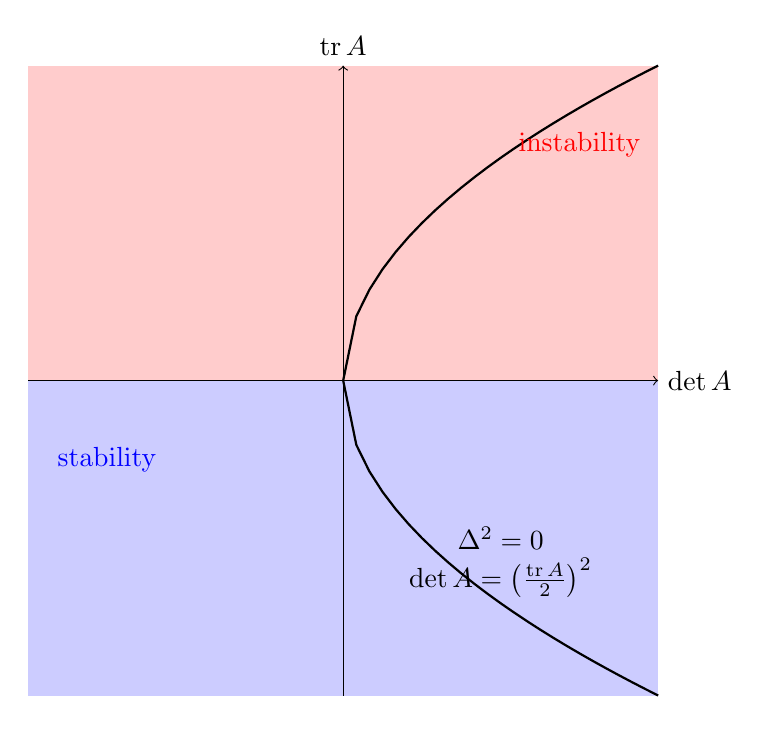
\begin{tikzpicture}
    % Set the size of the grid and the colors
    \fill[red!20] (-4,0) rectangle (4,4);
    \fill[blue!20] (-4,-4) rectangle (4,0);
    
    % Draw the axes
    \draw[->] (-4,0) -- (4,0) node[right] {$\det A$};
    \draw[->] (0,-4) -- (0,4) node[above] {$\operatorname{tr} A$};
    
    % Draw the parabola
    \draw[thick, domain=0:4] plot (\x, {sqrt(\x*4)}) node[right] {};
    \draw[thick, domain=0:4] plot (\x, {-sqrt(\x*4)}) node[right] {};
    
    % Stability and Instability regions
    \node[blue] at (-3,-1) {stability};
    \node[red] at (3,3) {instability};
    
    % Label for the critical point
    \node at (2, -2) {$\Delta^2=0$};
    \node at (2, -2.5) {$\det A = \left(\frac{\operatorname{tr} A}{2}\right)^2$};
\end{tikzpicture}

\citep{murray}


\newpage
    
    
    \bibliography{bibliography.bib}
    \medskip
    \newline
    \noindent
    \textbf{A note to the bibliography.}
    This assignment specifically focuses on Turing patterns in \textit{networks}, with recommendation to replicate the findings presented in \cite{main_network}. However, for someone unfamiliar with Turing patterns, a few preliminary read may be necessary. Article \cite{bio_article}, targeted at biologists, offers an intuitive overview of the concept with minimal mathematical details. To delve deeper into the mathematical foundations, \cite[][\textit{Chapter 2: Spatial Pattern Formation with Reaction Diffusion Systems}]{murray} provides a comprehensive and detailed explanation of Turing Patterns in a continuous medium. Another valuable resource is \cite[][\textit{Chapter 7: The Turing Model for Biological Pattern Formation}]{altbook}, which, while shorter than Murray’s chapter, still offers insightful observations.    
\end{document}


